\begin{figure*}[t]
  \centering
  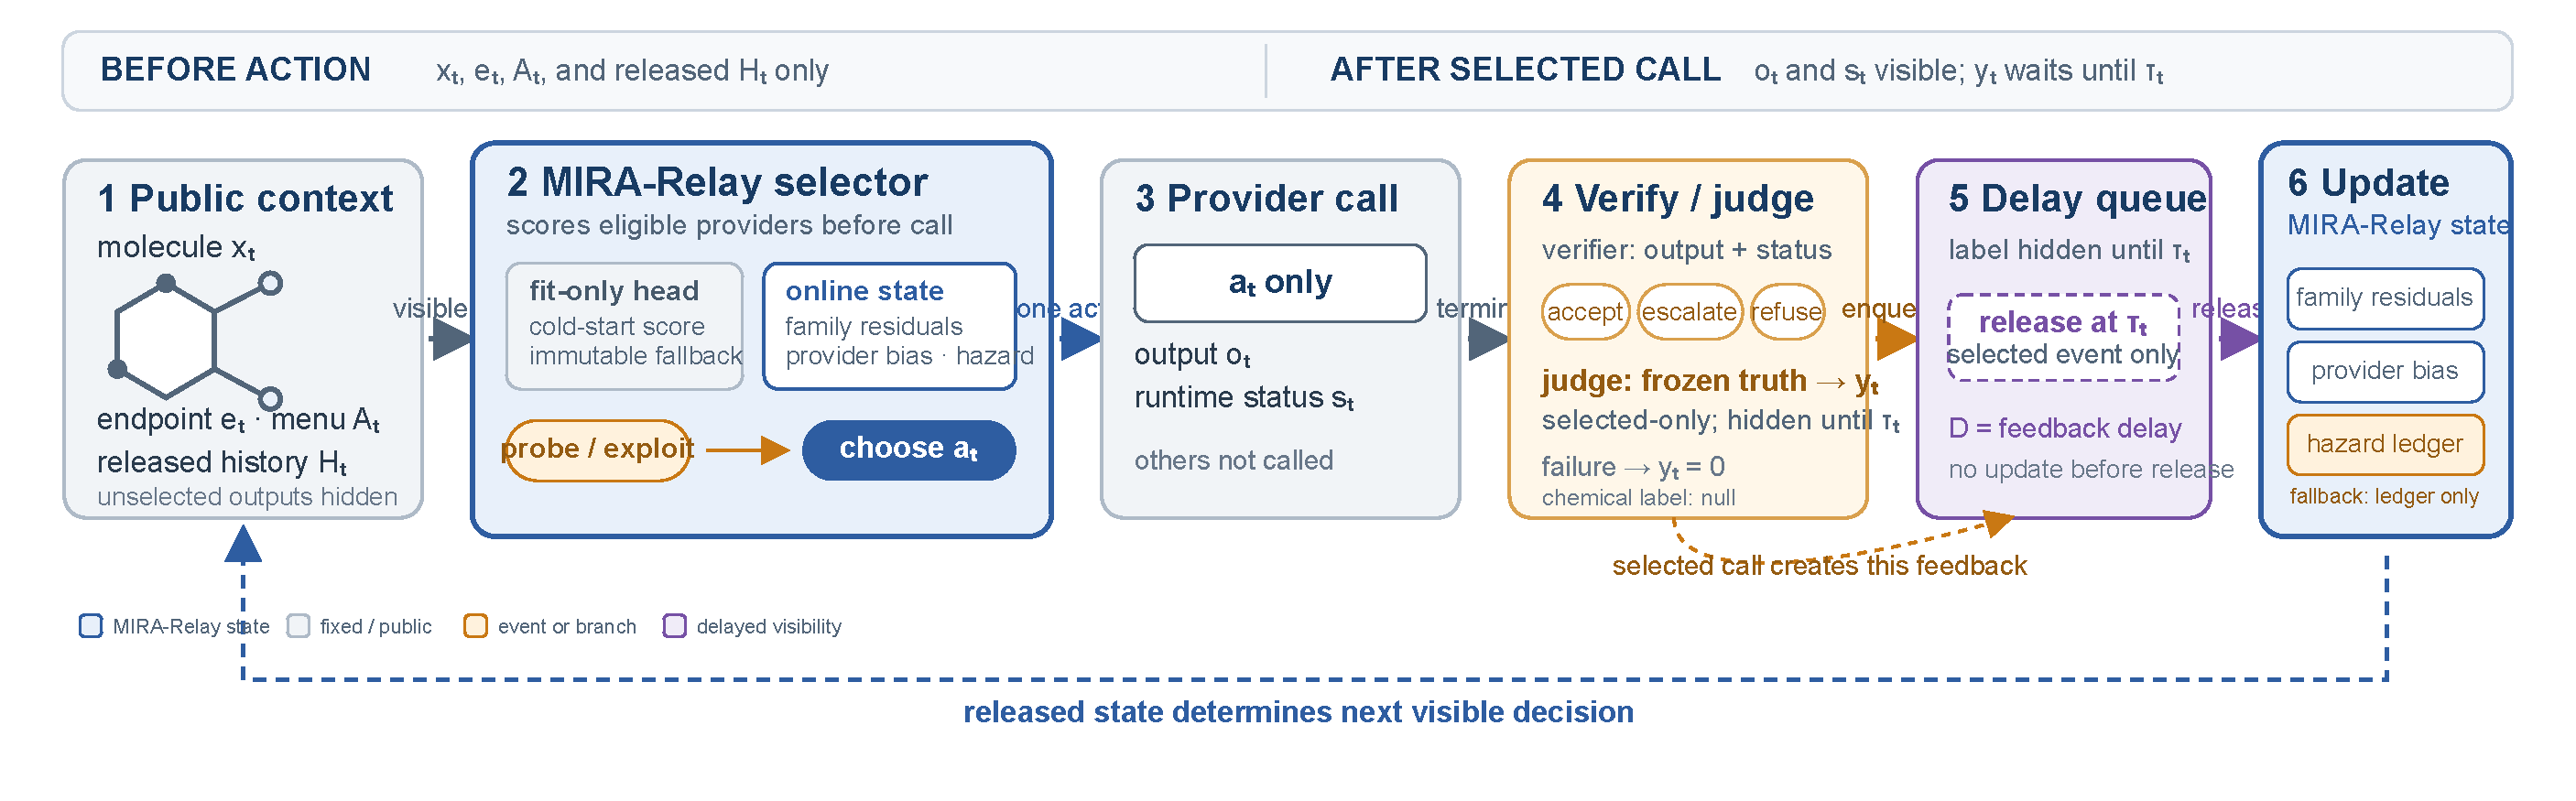
\includegraphics[width=\textwidth]{figures/figure1/v3/figure1_v3.pdf}
  \caption{MIRA-Relay turns tool selection into a delayed event loop. Before action, the selector sees the molecule, endpoint, current provider menu, and released history, then chooses one provider using a fit-only fallback and the online family/provider state. The runtime verifier handles the selected output and status; an independent frozen endpoint judge creates the selected-only label, which updates the shared challenger state only at its release tick. The fallback keeps its fit-only action score and receives ledger bookkeeping only.}
  \Description{A left-to-right framework with public molecule and provider-menu context; a MIRA-Relay selector with fit-only head, family residuals, provider bias, and probe/exploit; one provider call; a post-call runtime verifier plus independent frozen endpoint judge; selected-only delayed feedback; and a shared state update with a fallback ledger-only exception.}
  \label{fig:overview}
\end{figure*}
